\documentclass[tikz,border=2pt]{standalone}
\usepackage{amsmath,amssymb}
\usepackage{pgfplots}
\pgfplotsset{compat=1.18}
\usetikzlibrary{arrows.meta}
\begin{document}
% Reporting decision: reporting brings the reimbursement (line y = x, x = reimbursement) but raises expected discounted future
% premiums by 120; losses below 120 are kept unreported (80: gain 80 < 120), larger ones reported (200 > 120).
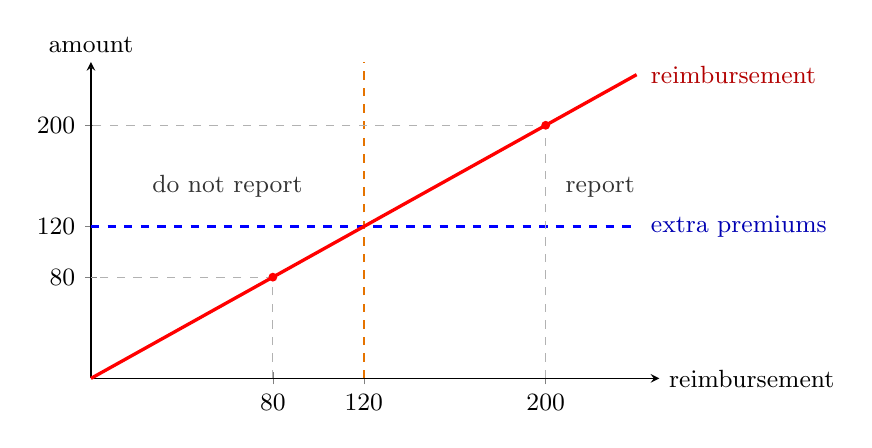
\begin{tikzpicture}[font=\small, >={Latex[length=2mm]}]
  \begin{axis}[
    axis lines=left, xmin=0, xmax=250, ymin=0, ymax=250,
    xtick={80,120,200}, ytick={80,120,200},
    xlabel={reimbursement}, ylabel={amount},
    xlabel style={at={(axis description cs:1,0)}, anchor=west},
    ylabel style={rotate=-90, at={(axis description cs:0,1)}, anchor=south},
    width=8.8cm, height=5.6cm, clip=false
    ]
    \draw[orange!90!black, thick, dashed] (axis cs:120,0) -- (axis cs:120,250);
    \addplot[blue, very thick, dashed, domain=0:240, samples=2] {120};
    \addplot[red, very thick, domain=0:240, samples=2] {x};
    \draw[gray!60, thin, dashed] (axis cs:80,0) -- (axis cs:80,80) -- (axis cs:0,80);
    \draw[gray!60, thin, dashed] (axis cs:200,0) -- (axis cs:200,200) -- (axis cs:0,200);
    \fill[red] (axis cs:80,80) circle (1.6pt);
    \fill[red] (axis cs:200,200) circle (1.6pt);
    \node[red!70!black, anchor=west] at (axis cs:242,240) {reimbursement};
    \node[blue!70!black, anchor=west] at (axis cs:242,120) {extra premiums};
    \node[gray!40!black, anchor=south] at (axis cs:60,135) {do not report};
    \node[gray!40!black, anchor=south] at (axis cs:224,135) {report};
  \end{axis}
\end{tikzpicture}
\end{document}
